\documentclass[symmetric]{tufte-handout}

%\geometry{showframe}% for debugging purposes -- displays the margins

\usepackage{amsmath}
\usepackage{mathtools}
\usepackage{amsfonts}
\usepackage{amsthm}


\usepackage{microtype}


% Set up the images/graphics package
\usepackage{graphicx}
\setkeys{Gin}{width=\linewidth,totalheight=\textheight,keepaspectratio}
\graphicspath{{graphics/}}

\title{Lecture Notes -- The Julia Set}
\author{Josh Lipschultz \& Ricky LeVan}
\date{}  % if the \date{} command is left out, the current date will be used

% The following package makes prettier tables.  We're all about the bling!
\usepackage{booktabs}

% The units package provides nice, non-stacked fractions and better spacing
% for units.
\usepackage{units}

% The fancyvrb package lets us customize the formatting of verbatim
% environments.  We use a slightly smaller font.
\usepackage{fancyvrb}
\fvset{fontsize=\normalsize}

% Small sections of multiple columns
\usepackage{multicol}

% Provides paragraphs of dummy text
\usepackage{lipsum}

% These commands are used to pretty-print LaTeX commands
\newcommand{\doccmd}[1]{\texttt{\textbackslash#1}}% command name -- adds backslash automatically
\newcommand{\docopt}[1]{\ensuremath{\langle}\textrm{\textit{#1}}\ensuremath{\rangle}}% optional command argument
\newcommand{\docarg}[1]{\textrm{\textit{#1}}}% (required) command argument
\newenvironment{docspec}{\begin{quote}\noindent}{\end{quote}}% command specification environment
\newcommand{\docenv}[1]{\textsf{#1}}% environment name
\newcommand{\docpkg}[1]{\texttt{#1}}% package name
\newcommand{\doccls}[1]{\texttt{#1}}% document class name
\newcommand{\docclsopt}[1]{\texttt{#1}}% document class option name



\newtheorem{theorem}{Theorem}
\newtheorem{corollary}{Corollary}
\newtheorem{definition}{Definition}


\begin{document}

\maketitle% this prints the handout title, author, and date

\section{Preliminaries}\label{sec:problem-1}

As a quick recap of what we saw last week, recall the following facts.

The \textsl{stable set} of a a complex polynomial $P: \mathbb{C} \rightarrow \mathbb{C}$, denoted $S(P)$, is the complement of $J(C)$.

Another useful definition was that of a \textsl{bounded orbit}. An orbit is bounded if there exists a $K$ such that $|Q_c^{\circ n}(z)| < K$ for all $n$. Otherwise the orbit is \textsl{unbounded}.

The previous group also discussed how the points of $S^1$ were \textsl{supersensitive}. That is, any open ball $B$ around $z \in S^1$ has the property that $\bigcup_{n=0}^\infty Q_0^{\circ n} (B) = \mathbb{C} \setminus \{p\}$ for at most one point $p$.

We also defined the Julia Set $J_c$ as the boundary of the filled Julia set $K_c$. (The filled Julia set is the set of bounded points of $Q_c$.) We could alternatively define $J_c$ as the closure of the set of repelling points of $Q_c$ (in fact, this definition isn't limited to the quadratic map; any polynomial will do, and is denoted $J(P)$ ).

For the quadratic map $Q_0(z) = z^2$ we saw chaotic behavior only on $S^1$ by angle doubling ($\theta \rightarrow 2\theta$). We also saw that $|Q_0(z)| \rightarrow \infty$ for all $|z| > 1$ and $|Q_0(z)| \rightarrow 0$ for all $|z| < 1$.

Finally, we learned that for $Q_{-2}(z) = z^2 - 2$, we have $J_2 = K_2 = [-2, 2]$, so any $z \in \mathbb{C} \ [-2,2] \rightarrow \infty$ as we compose $Q_{-2}(z)$ infinitely many times. 


\section{16.3 -- The Julia Set as a Cantor Set}\label{sec:problem-1}

Our goal for this section of the talk is to discuss and prove parts of
the following theorem.


\begin{theorem}
If $|c|$ is sufficiently large, $\Lambda$, the set of points whose entire forward orbits lie within the circle $|z|=|c|$, is a Cantor set on which $Q_c$ is topologically conjugate to the shift map on two symbols. All points in $\mathbb{C} - \Lambda$ tend to $\infty$ under iteration of $Q_c$. Hence, $J_c=K_c$.
\end{theorem}



\subsection{Points Which Escape}



\begin{theorem} \label{escape} [The Escape Criterion]
Suppose $2 < |c| \le |z|$. Then we have that $|Q_c^n(z)| \rightarrow \infty$ as $n \rightarrow \infty$.

\end{theorem}
\begin{proof}
We use the triangle inequality to get the following estimate:
\begin{equation}
    |Q_c^n(z)| \geq |z|^2 - |c| \geq |z|^2 - |z| = |z|(|z|-1)
\end{equation}
Since $|z| > 2$, we know that $|z|-1>1$, so there exists $\lambda > 0$ such that 
\begin{equation}
    |Q_c^n(z)| \geq (1+\lambda)^n|z|
\end{equation}
Since $|z|$ is fixed and $(1+\lambda)^n$ grows arbitrarily large, $|Q_c^n(z)|$ also grows arbitrarily large, as desired.

\end{proof}




\subsection{Points Which Escape}




\subsection{The Filled Julia Set}

\begin{theorem}
Let $D$ be the closed disk (i.e. $\{z : |z| \le |c|\}$), with $|c|>2$. Then the filled Julia set of $Q_c$ is given by
\begin{align*}
K_c = \bigcap\limits_{n\ge 0} Q_c^{\circ -n} (D)
\end{align*}
where $Q_c^{\circ -n} (D)$ denotes the preimage of $D$ under $Q_c^{\circ n}$
\end{theorem}

\begin{proof}
    Consider the case where
    $z\notin \bigcap_{n\ge 0} Q_c^{\circ -n} (D)$.
    Then there exists some $k\in \mathbb{N}$ such that $z\notin Q_c^{\circ -k} (D)$,
    so we have that $Q_c^{\circ k}(z) \notin D$. 
    Thus by Theorem~\ref{escape}, $z$ escapes to infinity under iteration
    of $Q_c$, so $z\notin K_c$.  

    Otherwise, if $z\in \bigcap_{n\ge 0} Q_c^{\circ -n} (D)$, then 
     $Q_c^{\circ n}(z) \in D$ for all $n\in \mathbb{N}$. Thus $z$ is bounded under
     iteration of $Q_c$, so $z\in K_c$.
\end{proof}

\marginnote{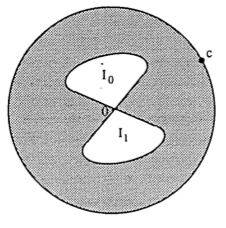
\includegraphics{lobes1.png}}
\newthought{The above characterization} of Julia sets provides a method of construction based on 
a given function $Q_c$. The key idea is that inverting the quadratic function and 
applying the Boundary Mapping Principle gives us a system of nested ``figure-eight''
lobes within lobes.

More specifically, begin with a disk of radius $|c|$ centered at the origin. We can take reverse-iterations of $Q_c$ by subtracting $c$ from all points, then taking their square root. The shape this process yields is one similar to the picture on the left. The lemniscate-like shape has two lobes, each of which has a diffeomorphic mapping to the entire 

\marginnote{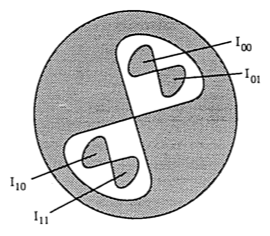
\includegraphics{lobes2.png}}


% Section 16.4
\section{16.4 -- Computing the Filled Julia Set}\label{sec:problem-1}










% Section 16.6
\section{16.6 -- Computing the Julia Set Another Way}\label{sec:problem-1}





\end{document}
